\documentclass[../main.tex]{subfiles}

\begin{document}

\section{Earth's gravitational field and other perturbations}\label{sec:force}
So far we have only considered the gravitational force acting between point masses. In reality, the Earth is not a point mass, neither a spherically symmetric mass distribution. In this section we will delve into the details of a more realistic model of the Earth's gravitational field.
\subsection{Geopotential model}
\subsubsection{Continuous distribution of mass}
In \cref{sec:twoBody} we saw that the motion of a body orbiting another one can be described by a conic section. However, we have not been concerned about the mass distribution of the large body, in our case the Earth. In this section we will see that the motion of the smaller body, the satellite, is slightly perturbed by the mass distribution of the Earth as well as the presence of other forces such as atmospheric drag, solar radiation pressure, or the gravitational pull of the Moon and Sun, which we will discuss later on. Nevertheless, the perturbations are relatively small and the orbits of the satellites are still approximating ellipses, but as we will corroborate experimentally in \cref{sec:simulation} these perturbations are essential to obtain accurate results.

Consider a body confined in a compact region $\Omega\subseteq\RR$ with a continuous density of mass $\rho:\Omega\to\RR$. We would like to know the gravitational pull on a point mass $m$ located at position $\vf{r}$ from the center of mass of the body. To do this, consider a covering of $\Omega$ in a set of disjoint cubes $Q_i$, $i=1,\dots,N$, small enough to be considered as point masses and let $R_i:=Q_i\cap \Omega$. Then, $\bigsqcup_{i=1}^NR_i=\Omega$. If each $R_i$ has mass $m_i$, volume $V_i$, density $\rho_i$, and its center is located at $\vf{s}_i\in\RR^3$, then the total gravitational acceleration $\vf{g}$ exerted on $m$ is the sum of the contributions of all the forces exerted by the $N$ point masses, and it is given by:
\begin{equation}\label{eq:riemann_sum}
  \vf{g}=-\sum_{i=0}^{N}\frac{m_{i}}{\norm{\vf{r}-\vf{s}_{i}}^3}(\vf{r}-\vf{s}_{i})=-\sum_{i=0}^{N}\frac{\rho_{i}}{\norm{\vf{r}-\vf{s}_{i}}^3}(\vf{r}-\vf{s}_{i})V_i
\end{equation}
Note that \cref{eq:riemann_sum} is a Riemann sum and so letting $N\to\infty$ we get:
\begin{equation}\label{eq:limit}
  \vf{g}=-\int_{\Omega}\frac{\rho(\vf{s})}{\norm{\vf{r}-\vf{s}}^3}(\vf{r}-\vf{s})\dd^3{\vf{s}}
\end{equation}
where $\dd^3{\vf{s}}:=\dd{x'}\dd{y'}\dd{z'}$, if $\vf{s}=(x',y',z')$.
% Consider a body confined in a compact region $\Omega\subseteq\RR$ with a continuous density of mass $\rho:\Omega\to\RR$. We would like to know the gravitational pull on a point mass $m$ located at position $\vf{r}$ from the center of mass of the body. To do this we can discretize the body $\Omega$ in a set of cubes $Q_{i,j,k}$ each of mass $m_{i,j,k}$, volume $\frac{1}{n_xn_yn_z}$ and density $\rho\left(\frac{i}{n_x},\frac{j}{n_y},\frac{k}{n_z}\right)=:\rho_{i,j,k}$, where $n_x$, $n_y$, and $n_z$ are the number of cubes in the $x$, $y$, and $z$ directions, respectively. The total gravitational acceleration $\vf{g}$ exerted on $m$ is the sum of the contributions of all the forces exerted by the cubes (considered as point masses) and it is given by:
% \begin{equation}\label{eq:riemann_sum}
%   \vf{g}=-\sum_{i=0}^{n_x}\sum_{j=0}^{n_y}\sum_{k=0}^{n_z}\frac{m_{i,j,k}}{\norm{\vf{r}-\vf{s}_{i,j,k}}^3}(\vf{r}-\vf{s}_{i,j,k})=-\sum_{i=0}^{n_x}\sum_{j=0}^{n_y}\sum_{k=0}^{n_z}\frac{\rho_{i,j,k}}{\norm{\vf{r}-\vf{s}_{i,j,k}}^3}(\vf{r}-\vf{s}_{i,j,k})\frac{1}{n_xn_yn_z}
% \end{equation}
% where $\vf{s}_{i,j,k}=(\frac{i}{n_x},\frac{j}{n_y},\frac{k}{n_z})$ (in Cartesian coordinates). Note that \cref{eq:riemann_sum} is a Riemann sum and so letting $n_x,n_y,n_z\to\infty$ we get:
% \begin{equation}\label{eq:limit}
%   \vf{g}=-\int_{\Omega}\frac{\rho(\vf{s})}{\norm{\vf{r}-\vf{s}}^3}(\vf{r}-\vf{s})\dd^3{\vf{s}}
% \end{equation}
% where $\dd^3{\vf{s}}:=\dd{x'}\dd{y'}\dd{z'}$, if $\vf{s}=(x',y',z')$.
\begin{restatable}{theorem}{thmconservative}\label{thm:conservative}
  Let $\Omega$ be a compact region in $\RR^3$ with a continuous density of mass $\rho:\Omega\to\RR$. Then, the gravitational acceleration field $\vf{g}$ is conservative. That is, there exists a function $f:\RR^3\rightarrow\RR$ such that $\vf{g}=\grad f$.
\end{restatable}
\begin{proof}
  See \cref{sec:app3}.
\end{proof}
% \begin{theorem}\label{thm:conservative}
%   Let $\Omega$ be a compact region in $\RR^3$ with a continuous density of mass $\rho:\Omega\to\RR$. Then, the gravitational acceleration field $\vf{g}$ is conservative. That is, there exists a function $f:\RR^3\rightarrow\RR$ such that $\vf{g}=\grad f$.
% \end{theorem}
Physically speaking, the gravitational force $\vf{F}$ being conservative means that the work $W$ done by the force along a path $C$
\begin{equation}
  W=\int_C\vf{F}\cdot\dd{\vf{s}}
\end{equation}
depends only on the initial and final positions of it. Moreover, due to historical reasons, we will write $\vf{g}=-\grad V$ (with the minus sign) and call $V$ the \emph{gravitational potential}. The minus sign is chosen according the convention that work done by gravitational forces decreases the potential.
\subsubsection{Laplace's equation for \texorpdfstring{$V$}{V}}\label{sec:laplace}
\begin{restatable}{theorem}{thmlaplace}\label{thm:laplace}
  Consider a distribution of matter of density $\rho$ in a compact region $\Omega$. Then, the gravitational potential $V$ satisfies the Laplace equation
  \begin{equation}
    \laplacian V = 0
  \end{equation}
  for all points outside $\Omega$\footnote{It can be seen that $V$ satisfies in fact the \emph{Poisson equation} $\laplacian V=4\pi G\rho$ for any point $\vf{r}\in\RR^3$, which reduces to Laplace equation when $\vf{r}\in\Omega^c$, because there we have $\rho(\vf{r})=0$.}.
\end{restatable}
\begin{proof}
  See \cref{sec:app3}.
\end{proof}
% \begin{theorem}
%   Consider a distribution of matter of density $\rho$ in a compact region $\Omega$. Then, the gravitational potential $V$ satisfies the Laplace equation
%   \begin{equation}
%     \laplacian V = 0
%   \end{equation}
%   for all points outside $\Omega$\footnote{It can be seen that $V$ satisfies in fact the \emph{Poisson equation} $\laplacian V=4\pi G\rho$ for any point $\vf{r}\in\RR^3$, which reduces to Laplace equation when $\vf{r}\in\Omega^c$, because there we have $\rho(\vf{r})=0$.}.
% \end{theorem}
So far we have seen that the gravitational potential $V$ satisfies the Laplace equation. If, moreover, we choose the origin of potential to be at the infinity, that is, if we impose $\displaystyle\lim_{\norm{\vf{r}}\to\infty}V=0$, then the gravitational potential created by a distribution of mass in a compact region $\Omega$ is a solution of the following exterior Dirichlet problem:
\begin{equation}\label{eq:dirichletProblem}
  \begin{cases}
    \laplacian V = 0 & \text{in } \Omega^c    \\
    V = f            & \text{on } \Fr{\Omega} \\
    \displaystyle\lim_{\norm{\vf{r}}\to\infty}V=0
  \end{cases}
\end{equation}
If $\Omega$ represents the Earth, then $f=f(\theta,\phi)$ is the boundary condition concerning the gravitational potential at the surface of the Earth as a function of the longitude $\theta$ and colatitude $\phi$.

We will see now that \cref{eq:dirichletProblem} has a unique solution. To do that we invoke the maximum principle, which we will not prove here (see \cite{evans} for more details).
\begin{theorem}[Maximum principle]
  Let $U\subset \RR^n$ be open and bounded and $u\in\mathcal{C}^2(U)\cap \mathcal{C}(\overline{U})$. Suppose that $u$ is harmonic within $U$, that is, $\laplacian u=0$ in $U$. Then, $\max_{\overline{U}}u=\max_{\partial U}u$.
\end{theorem}
\begin{restatable}{theorem}{Dirichlet}\label{thm:max_principle}
  The Dirichlet problem of \cref{eq:dirichletProblem} has a unique solution.
\end{restatable}
\begin{proof}
  See \cref{sec:app3}.
\end{proof}
% \begin{corollary}
%   The Dirichlet problem of \cref{eq:dirichletProblem} has a unique solution.
% \end{corollary}
Now that we know that the Dirichlet problem has a unique solution, we can proceed to find it. In the next section we will construct an explicit solution for the gravitational potential created by the Earth.
\subsection{Spherical harmonics}
\subsubsection{Legendre polynomials, regularity and orthonormality}
In this section we aim to introduce a class of functions that will appear later on in the general solution of the Laplace equation (see \cref{sec:laplace_spherical}). To accomplish this, we need first to introduce the Legendre polynomials. There are several ways to define them, but the most convenient one for our purposes is from the following differential equation. Consider the following second-order differential equation called \emph{Legendre differential equation}:
\begin{equation}
  (1-x^2)y''-2xy'+\lambda y=0
\end{equation}
for $\lambda\in\RR$. This equation can be rewritten as:
\begin{equation}\label{eq:legendre_diff_eq}
  {((1-x^2)y')}'+\lambda  y=0
\end{equation}
Seeking for analytic solutions of this equation using the power series method \cite{florida:legendre}, i.e.\ looking for solutions of the form $y(x)=\sum_{j=0}^{\infty}a_jx^j$, we see that:
\begin{multline}
  0=(1-x^2)\sum_{j=2}^{\infty}a_{j}(j-1)jx^{j-2}-2x\sum_{j=1}^{\infty}a_{j}jx^{j-1}+\lambda\sum_{j=0}^{\infty}a_jx^j =\sum_{j=0}^{\infty}a_{j+2}(j+1)(j+2)x^j-\\-\sum_{j=0}^{\infty}a_{j}(j-1)jx^{j}-\sum_{j=0}^{\infty}2a_{j}jx^{j}+\sum_{j=0}^{\infty}\lambda a_jx^j  =\sum_{j=0}^{\infty}[a_{j+2}(j+1)(j+2) - a_j(j(j+1)-\lambda)]x^j
\end{multline}
Equating the general term of the series to 0 we obtain this recursion:
\begin{equation}\label{eq:legendre_recursion}
  a_{j+2}=\frac{j(j+1)-\lambda}{(j+1)(j+2)}a_j\quad j=0,1,2,\ldots
\end{equation}
From here we can obtain two independent solutions by setting the initial conditions $a_0$ and $a_1$ of the iteration. For example, setting $a_1=0$ we obtain a series that has only even powers of $x$. On the other hand, setting $a_0=0$ we obtain a series that has only odd powers of $x$. These two series converge on the interval $(-1,1)$ by the ratio test (by looking at \cref{eq:legendre_recursion}) and can be expressed compactly as \cite{florida:legendre}:
\begin{equation}\label{eq:legendre_series}
  y_\mathrm{e}(x)=a_0\sum_{j=0}^{\infty}\left[\prod_{k=0}^{j-1}(2k(2k+1)-\lambda)\right]\frac{x^{2j}}{(2j)!}\quad y_\mathrm{o}(x)=a_1\sum_{j=0}^{\infty}\left[\prod_{k=0}^{j-1}((2k+1)(2k+2)-\lambda)\right]\frac{x^{2j+1}}{(2j+1)!}
\end{equation}
Here, the empty product (that is, when $k$ ranges from 0 to $-1$) is defined to be 1. However, for each $\lambda\in\RR$ either one of these series or both diverge at $x=\pm 1$, as they behave as the harmonic series in a neighborhood of $x=\pm 1$. We are interested, though, in the solutions that remain bounded on the whole interval $[-1,1]$. Looking at the expressions of \cref{eq:legendre_series} one can check that the only possibility to make the series converge in $[-1,1]$ is when $\lambda =n(n+1)$, $n\in\NN\cup\{0\}$. In this case, for each $n\in\NN\cup\{0\}$ exactly one of the series is in fact a polynomial of degree $n$. If, furthermore, we choose $a_0$ or $a_1$ be such that the polynomial evaluates to 1 at $x=1$, these polynomials are called \emph{Legendre polynomials}, and they are denoted by $P_n(x)$. The other (divergent) series is usually denoted in the literature by $Q_n(x)$ (check \cite{mathematical_methods,florida:legendre}) and it is independent of $P_n(x)$. Thus, the general solution of \cref{eq:legendre_diff_eq} for $\lambda=n(n+1)$ can be expressed as a linear combination of $P_n$ and $Q_n$, because the space of solutions form a vector space of dimension 2.
\begin{center}
  \centering
  \begin{minipage}[ht]{0.47\textwidth}
    \centering
    % \captionsetup{type=table} %% tell latex to change to table
    \begin{tabular}{|c|c|}
      \hline
      $n$ & $P_n(x)$                                 \\
      \hline\hline
      $0$ & $1$                                      \\
      $1$ & $x$                                      \\
      $2$ & $\frac{1}{2}(3x^2-1)$                    \\
      $3$ & $\frac{1}{2}(5x^3-3x)$                   \\
      $4$ & $\frac{1}{8}(35x^4-30x^2+3)$             \\
      $5$ & $\frac{1}{8}(63x^5-70x^3+15x)$           \\
      $6$ & $\frac{1}{16}(231x^6-315x^4+105x^2-5)$   \\
      $7$ & $\frac{1}{16}(429x^7-693x^5+315x^3-35x)$ \\
      \hline
    \end{tabular}
    \captionof{table}{First eight Legendre polynomials}
    \label{tab:legendre_polys}
  \end{minipage}
  \hspace{0.02\textwidth}
  \begin{minipage}[ht]{0.47\textwidth}
    \centering
    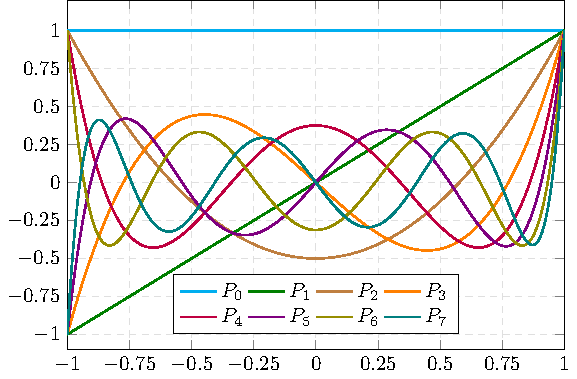
\includegraphics[width=\textwidth]{Images/legendre.pdf}
    \captionof{figure}{Graphic representation of the first eight Legendre polynomials.}
  \end{minipage}
\end{center}
% The following proposition gives and explicit formula for the Legendre polynomials.
% \begin{proposition}[Rodrigues' formula]
%   Let $n\in \NN\cup\{0\}$. Then, $\forall x\in[-1,1]$:
%   \begin{equation}\label{eq:rodrigues}
%     P_n(x)=\frac{1}{2^n n!}\dv[n]{}{x}\left[{\left(x^2-1\right)}^n\right]
%   \end{equation}
% \end{proposition}
% \textcolor{red}{\begin{proposition}
%     Consider the function $g_x(t)=\frac{1}{\sqrt{1-2xt+t^2}}$ with $\abs{x}\leq 1$. Then, the generating function of $g$ is:
%     \begin{equation}
%       \frac{1}{\sqrt{1-2xt+t^2}}=\sum_{n=0}^{\infty}P_n(x)t^n
%     \end{equation}
%   \end{proposition}
%   \begin{proof}
%     Assume that formally $\frac{1}{\sqrt{1-2xt+t^2}}=\sum_{n=0}^{\infty}Q_n(x)t^n$. We want to check that $Q_n(x)=P_n(x)$ for all $n\in\NN\cup\{0\}$. Differentiating the equation with respect to $x$ and with respect to $t$ we obtain:
%     \begin{equation}\label{eq:rec_legendre_proof}
%       \frac{x-t}{{(1-2xt+t^2)}^{3/2}}=\sum_{n=0}^{\infty}nQ_n(x)t^{n-1}\qquad\frac{t}{{(1-2xt+t^2)}^{3/2}}=\sum_{n=0}^{\infty}{Q_n}'t^n
%     \end{equation}
%     The second equation can be rewritten as:
%     \begin{equation}
%       t\sum_{n=0}^{\infty}Q_n t^n=(1-2xt+t^2)\sum_{n=0}^{\infty}{Q_n}'(x)t^{n-1}
%     \end{equation}
%     So equating the coefficients of $t^n$ we get:
%     \begin{equation}
%       Q_{n}={Q_{n+1}}'-2x{Q_n}'+{Q_{n-1}}'
%     \end{equation}
%     Moreover, from \cref{eq:rec_legendre_proof} we have that:
%     \begin{equation}
%       t\sum_{n=0}^{\infty}nQ_n(x)t^{n-1}=(x-t)\sum_{n=0}^{\infty}{Q_n}'(x)t^{n}
%     \end{equation}
%     Again equating the coefficients of $t^n$ we get:
%     \begin{equation}
%       nQ_n=x{Q_n}'-{Q_{n-1}}'
%     \end{equation}
%     Hence differentiating $(1-x^2){P_n}'$ we have:
%     \begin{equation}
%       {((1-x^2){P_n}')}'=-2x{P_n}'+(1-x^2)P
%     \end{equation}
%     \textcolor{red}{NOT FINISHED!!!!!!!!!!}
%   \end{proof}}
The following proposition will be of our interest in the next section \cite{mathematical_methods}.
\begin{proposition}\label{prop:associate_legendre}
  Let $y(x)$ be a solution to the Legendre differential equation. Then, $\forall m\in\NN\cup\{0\}$ the function
  \begin{equation}
    w_m(x)={(1-x^2)}^{m/2} \dv[m]{y(x)}{x}
  \end{equation}
  solves the \emph{general Legendre differential equation}:
  \begin{equation}
    (1-x^2)y''-2xy'+\left(\lambda - \frac{m^2}{1-x^2}\right) y=0
  \end{equation}
  In particular if $\lambda=n(n+1)$ for $n\in\NN\cup\{0\}$, then $w_m(x)$ is denoted as
  \begin{equation}\label{eq:associated_legendre_polynomials}
    P_{n,m}(x):={(1-x^2)}^{m/2} \dv[m]{P_n}{x}
  \end{equation}
  and it is called the \emph{associated Legendre polynomial} of degree $n$ and order $m$.
\end{proposition}
% \begin{proof}
%   We know that $P_n$ satisfies the equation:
%   \begin{equation}\label{eq:proof_aso1}
%     (1-x^2)P_n''-2xP_n'+n(n+1)P_n=0
%   \end{equation}
%   Recall the Leibniz rule for differentiation:
%   \begin{equation}
%     {(fg)}^{(m)}=\sum_{k=0}^{m}\binom{m}{k}f^{(m-k)}g^{(k)}
%   \end{equation}
%   Differentiating \cref{eq:proof_aso1} $m$ times using the Leibniz rule and letting $v=\dv[m]{P_n}{x}$ we obtain:
%   \begin{equation}
%     [(1-x^2)v''-2xm v'-m(m-1)v]-[2xv'+2mv]+n(n+1)v= (1-x^2)v''-2x(m+1)v'+(n-m)(n+m+1)v=0
%   \end{equation}
%   Now let $P_{n,m}(x)={(1-x^2)}^{m/2}v$. Using the chain rule and isolating $v'$ and $v''$ we obtain:
%   \begin{align*}
%     {P_{n,m}}'= {(1-x^2)}^{m/2}v' - \frac{m}{2}x{(1-x^2)}^{m/2-1}v={(1-x^2)}^{m/2}v' - \frac{m}{2}\frac{P_{n,m}}{1-x^2}\implies v'= \frac{2}{m}\frac{1-x^2}{x}P_{n,m} - \frac{2}{m}x{P_{n,m}}' \\
%   \end{align*}
%   ....
% \end{proof}
Note that although we opted to call the functions $P_{n,m}$ as polynomials, they are only true polynomials when $m$ is even. But we have opted to call them in that manner as it is the common practice in the literature (see \cite{wolfram_associated_legendre_polynomials,mathematical_methods,florida:legendre}).

Moreover, from the definition of $P_{n,m}$, we can see that $P_{n,0}=P_n$ and that $P_{n,m}=0$ if $m>n$. So we can restrict the domain of $m$ to the set $\{0,1,\dots,n\}$.

% Finally, putting \cref{eq:associated_legendre_polynomials,eq:rodrigues} together, we obtain the following explicit formula for the associated Legendre polynomials:
% \begin{equation}
%   P_{n,m}(x)=\frac{1}{2^n n!}{(1-x^2)}^{m/2} \dv[n+m]{x}\left[{\left(x^2-1\right)}^n\right]
% \end{equation}
% This allows us to extend the range of $m$ to $\{-n,-(n-1),\dots,n-1,n\}$.
% \begin{lemma}\label{lem:neg_asso_legendre}
%   Let $n\in\NN\cup\{0\}$ and $m\in\{0,\ldots,n\}$. Then:
%   \begin{equation}
%     P_n^{-m}(x)=(-1)^m \frac{(n-m)!}{(n+m)!}P_{n,m}(x)
%   \end{equation}
% \end{lemma}
% This lemma shows us that the new extended associated polynomials $P_n^{-m}$, $m\in\{0,\ldots,n\}$, are also solutions to the general Legendre differential equation because the satisfy the same equation as $P_{n,m}$ and they only differ by a constant factor.
% My spherical harmonics are the same as the ones in Riley, Hobson, Bence except for the minus sign (-1)^m in front of Y_{n,m}^{\mathrm{c}}.  
\begin{table}[ht]
  \centering
  \captionsetup{type=table} %% tell latex to change to table
  \begin{tabular}{|c|c||c|c|}
    \hline
    $n$ & $P_{n,1}(x)$                              & $n$ & $P_{n,2}(x)$                          \\
    \hline
    $1$ & $\sqrt{1-x^2}$                            & $2$ & $3(1-x^2)$                            \\
    $2$ & $3x\sqrt{1-x^2}$                          & $3$ & $15x(1-x^2)$                          \\
    $3$ & $\frac{3}{2}(5 x^2-1)\sqrt{1-x^2}$        & $4$ & $\frac{15}{2}(7x^2-1)(1-x^2)$         \\
    $4$ & $\frac{5}{2}x(7x^2-3)\sqrt{1-x^2}$        & $5$ & $\frac{105}{2}x(3x^2-1)(1-x^2)$       \\
    $5$ & $\frac{15}{8}(21x^4-14x^2+1)\sqrt{1-x^2}$ & $6$ & $\frac{105}{8}(33x^4-18x^2+1)(1-x^2)$ \\
    \hline
  \end{tabular}
  \caption{First associated Legendre polynomials for $m=1$ and $m=2$.}
\end{table}
\begin{figure}[ht]
  \centering
  \begin{subfigure}[b]{0.48\textwidth}
    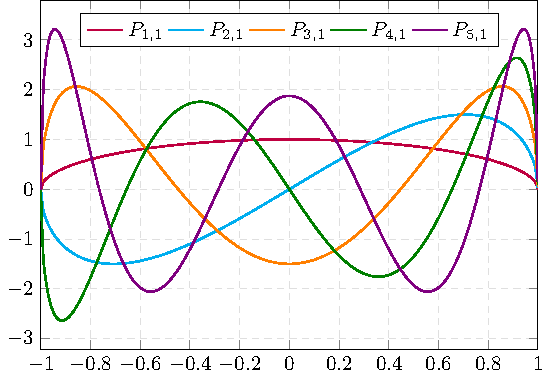
\includegraphics[width=\textwidth]{Images/assolegendre1.pdf}
    \caption{$m=1$}
  \end{subfigure}
  \quad
  \begin{subfigure}[b]{0.48\textwidth}
    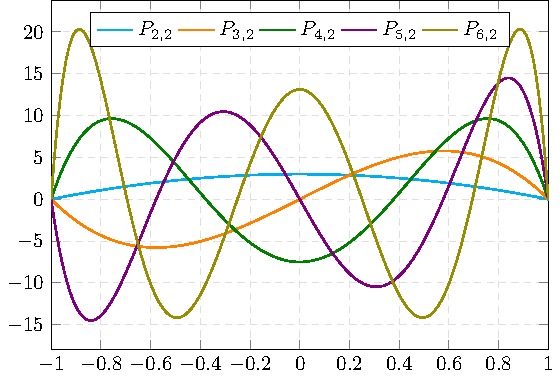
\includegraphics[width=\textwidth]{Images/assolegendre2.pdf}
    \caption{$m=2$}
  \end{subfigure}
  \caption{Graphic representation of the first associated Legendre polynomials for $m=1$ and $m=2$.}
\end{figure}
\begin{definition}
  Let $n\in\NN\cup\{0\}$ and $m\in\{0,1,\dots,n\}$. We define the \emph{real spherical harmonics} $Y_{n,m}^{\mathrm{c}}$ and $Y_{n,m}^{\mathrm{s}}$ as:
  \begin{align}
    Y_{n,m}^{\mathrm{c}}(\theta,\phi) & =\sqrt{(2-\delta_{0,m})(2n+1)\frac{(n-m)!}{(n+m)!} }P_{n,m}(\cos\phi) \cos{m\theta} \\
    Y_{n,m}^{\mathrm{s}}(\theta,\phi) & =\sqrt{(2-\delta_{0,m})(2n+1)\frac{(n-m)!}{(n+m)!} }P_{n,m}(\cos\phi) \sin{m\theta}
  \end{align}
  Here the coordinates $\theta\in [0,2\pi)$ and $\phi\in[0,\pi]$ are the spherical coordinates such that any point on the sphere can be written uniquely as $(x,y,z) = (\sin\phi\cos\theta,\sin\phi\sin\theta,\cos\phi)$. The factor $N_{n,m}:=\sqrt{(2-\delta_{0,m})(2n+1)\frac{(n-m)!}{(n+m)!} }$ is called the \emph{normalization factor} of the spherical harmonics and $\delta_{0,m}$ is the Kronecker delta and their appearance here will become clear in the next section.
\end{definition}
\begin{table}[ht]
  \centering
  \begin{tabular}{|c|c|c||c|c|c|}
    \hline
    $n$ & $m$ & $Y_{n,m}^{\mathrm{c}}(\theta,\phi)$     & $n$ & $m$ & $Y_{n,m}^{\mathrm{c}}(\theta,\phi)$                        \\
    \hline
    $0$ & 0   & $1$                                     & $2$ & 2   & $\frac{\sqrt{15}}{2}{(\sin\phi)}^2\cos 2\theta$            \\
    $1$ & 0   & $\sqrt{3}\cos\phi$                      & $3$ & 0   & $\frac{\sqrt{7}}{2}\cos\phi(5{(\cos\phi)}^2-3)$            \\
    $1$ & 1   & $\sqrt{3}\sin\phi\cos\theta$            & $3$ & 1   & $\frac{\sqrt{42}}{4}(5{(\cos\phi)}^2-1)\sin\phi\cos\theta$ \\
    $2$ & 0   & $\frac{\sqrt{5}}{2}(3{(\cos\phi)}^2-1)$ & $3$ & 2   & $\frac{\sqrt{105}}{2}{(\sin\phi)}^2\cos\phi\cos 2\theta$   \\
    $2$ & 1   & $\sqrt{15}\sin\phi\cos\phi\cos\theta$   & $3$ & 3   & $\frac{\sqrt{70}}{4}{(\sin\phi)}^3\cos 3\theta$            \\
    \hline
  \end{tabular}
  \caption{First cosine spherical harmonics.}
\end{table}
\begin{figure}[ht]
  \centering
  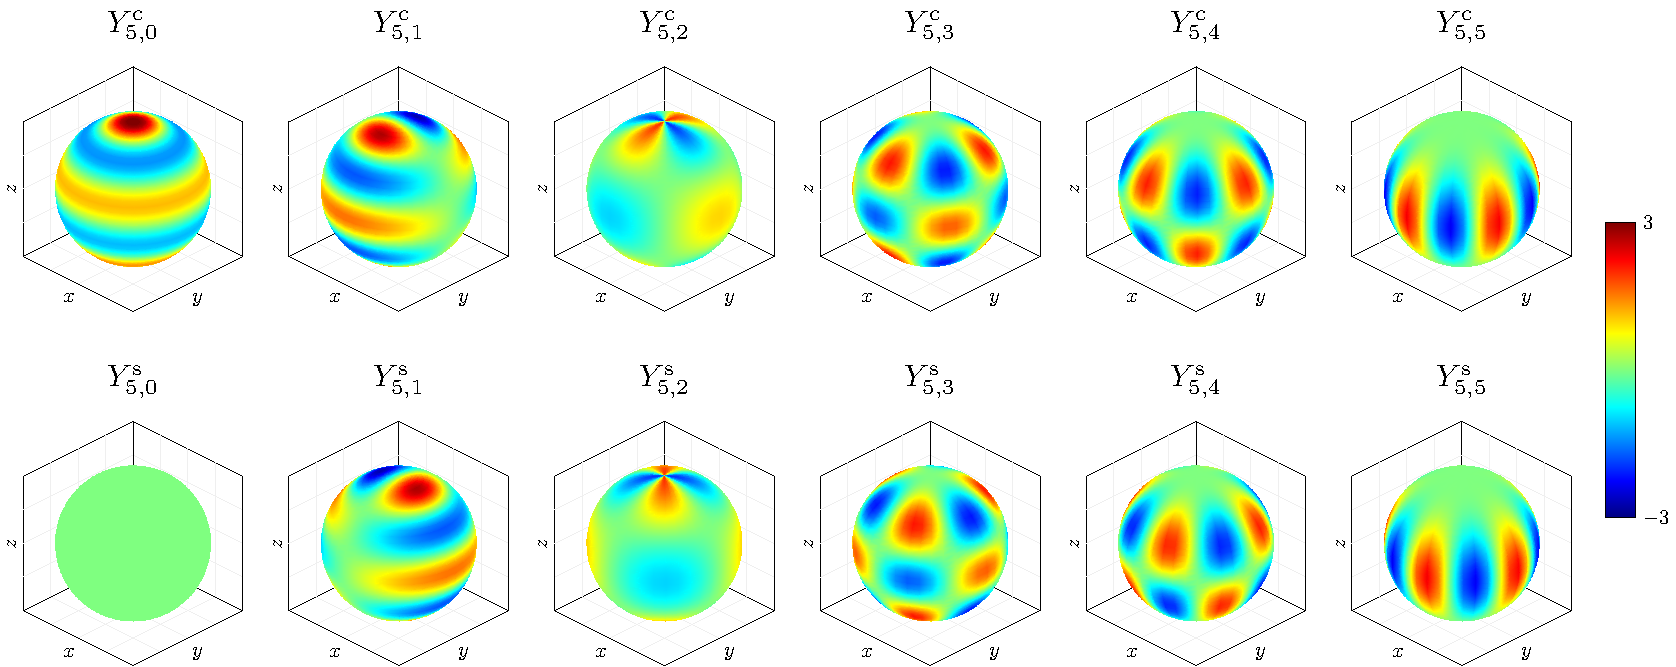
\includegraphics[width=\textwidth]{Images/sphericalHarmonics.pdf}
  \caption{3D color gradient representation of the spherical harmonics of degree $n=5$. The first row correspond to the cosine spherical harmonics and the second row correspond to the sine spherical harmonics.}
\end{figure}
The associated Legendre polynomials satisfy an orthogonality relation:
\begin{lemma}\label{lem:ortho_asso_legendre}
  Let $n_1,n_2\in\NN\cup\{0\}$ and $m\leq \min\{n_1,n_2\}$. Then:
  \begin{equation}
    \int_0^1 P_{n_1,m}(x) P_{n_2,m}(x) \dd{x}=\frac{2}{2n_1+1}\frac{(n_1+m)!}{(n_1-m)!} \delta_{n_1,n_2}
  \end{equation}
  where $\delta_{n_1,n_2}$ denotes the Kronecker delta.
\end{lemma}
Similarly, it can be shown that the spherical harmonics from an orthonormal family of functions:
\begin{restatable}{proposition}{propOrthoSphericalHarmonics}
  The family of spherical harmonics $\{Y_{n,m}^{\mathrm{c}}(\theta,\phi),Y_{n,m}^{\mathrm{s}}(\theta,\phi):n\in\NN\cup\{0\},m\leq n\}$ is orthonormal in the following sense:
  \begin{equation}\label{eq:ortho_spherical_harmonics}
    \frac{1}{4\pi}\int_0^{2\pi}\int_0^\pi Y_{n_1,m_1}^i(\theta,\phi) Y_{n_2,m_2}^j(\theta,\phi)\dd\Omega=\delta_{n_1,n_2}\delta_{m_1,m_2}\delta_{i,j}
  \end{equation}
  where $\dd\Omega=\sin\phi\dd{\phi}\dd{\theta}$ is the solid angle element, which measures the element of area on a sphere of radius $1$.
\end{restatable}
% \begin{proposition}
%   The family of spherical harmonics $\{Y_{n,m}^{\mathrm{c}}(\theta,\phi),Y_{n,m}^{\mathrm{s}}(\theta,\phi):n\in\NN\cup\{0\},m\leq n\}$ is orthonormal in the following sense:
%   \begin{equation}\label{eq:ortho_spherical_harmonics}
%     \frac{1}{4\pi}\int_0^{2\pi}\int_0^\pi Y_{n_1,m_1}^i(\theta,\phi) Y_{n_2,m_2}^j(\theta,\phi)\dd\Omega=\delta_{n_1,n_2}\delta_{m_1,m_2}\delta_{i,j}
%   \end{equation}
%   where $\dd\Omega=\sin\phi\dd{\phi}\dd{\theta}$ is the solid angle element, which measures the element of area on a sphere of radius $1$.
% \end{proposition}
Moreover, an important result in the Sturm-Liouville Theory of second order differential equations (\cite{wiki:sturmliouville,completenessSL}) says that the family of spherical harmonics $\{Y_{n,m}^{\mathrm{c}}(\theta,\phi),Y_{n,m}^{\mathrm{s}}(\theta,\phi):n\in\NN\cup\{0\},m\leq n\}$ form a complete set in the sense that any smooth function defined on the sphere $f:\mathrm{S}^2\rightarrow\RR$ can be expanded in a series of spherical harmonics:
\begin{equation}
  f(\theta,\phi)=\sum_{n=0}^\infty\sum_{m=0}^n (c_{n,m} Y_{n,m}^{\mathrm{c}}(\theta,\phi)+s_{n,m} Y_{n,m}^{\mathrm{s}}(\theta,\phi))
\end{equation}
This will be useful in \cref{sec:laplace_spherical_potential} when expanding the gravitational potential created by the Earth at some arbitrary point in spherical harmonics.
\subsubsection{Laplace's equation in spherical coordinates}\label{sec:laplace_spherical}
% \begin{definition}
%   Let $f:\RR^3\rightarrow\RR$ be a twice-differentiable function. The \emph{Laplace equation} is the equation:
%   \begin{equation}
%     \laplacian f=\pdv[2]{f}{x}+\pdv[2]{f}{y}+\pdv[2]{f}{z}=0
%   \end{equation}
% \end{definition}
We start first with this proposition that give us the laplacian of a function in spherical coordinates.
\begin{proposition}
  Let $f:\RR^3\rightarrow\RR$ be a twice-differentiable function. Then:
  \begin{equation}\label{eq:laplace}
    \laplacian f = \frac{1}{r^2}\pdv{}{r}\left(r^2\pdv{f}{r}\right)+\frac{1}{r^2\sin\phi}\pdv{}{\phi}\left(\sin\phi\pdv{f}{\phi}\right)+\frac{1}{r^2{(\sin\phi)}^2}\pdv[2]{f}{\theta}
  \end{equation}
  where $r\in[0,\infty)$ denotes the radial distance, $\theta\in[-\pi,\pi)$ denotes the longitude, and $\phi\in[0,\pi]$, the colatitude:
  \begin{equation}
    \begin{aligned}
      x & =r\sin\phi\cos\theta \\
      y & =r\sin\phi\sin\theta \\
      z & =r\cos\phi
    \end{aligned}
  \end{equation}
\end{proposition}
We are now interested in solving the Laplace equation. \cref{thm:laplace_spherical} gives the solution of it as a function of the spherical harmonics.
\begin{restatable}{theorem}{laplaceSolutions}
  \label{thm:laplace_spherical}
  The regular solutions in a bounded region $\Omega\subseteq \RR^3$ such that $0\notin\overline{\Omega}$ of the Laplace equation in spherical coordinates are of the form
  \begin{align}
    f(r,\theta,\phi) & = \sum_{n=0}^\infty \sum_{m=0}^n (a_n r^{n} +b_{n}r^{-n-1})P_{n,m}(\cos\phi) (c_{n,m}\cos(m\theta)+s_{n,m}\sin(m\theta))                                                              \\
                     & \label{eq:sol_laplace} = \sum_{n=0}^\infty \sum_{m=0}^n (a_n r^{n} +b_{n}r^{-n-1})(\tilde{c}_{n,m}Y_{n,m}^{\mathrm{c}}(\theta,\phi)+\tilde{s}_{n,m}Y_{n,m}^{\mathrm{s}}(\theta,\phi))
  \end{align}
  where $a_n,b_n,c_{n,m},s_{n,m},\tilde{c}_{n,m},\tilde{s}_{n,m}\in\RR$.
\end{restatable}
% \begin{theorem}\label{thm:laplace_spherical}
%   The regular solutions in a bounded region $\Omega\subseteq \RR^3$ such that $0\notin\overline{\Omega}$ of the Laplace equation in spherical coordinates are of the form
%   \begin{align}
%     f(r,\theta,\phi) & = \sum_{n=0}^\infty \sum_{m=0}^n (a_n r^{n} +b_{n}r^{-n-1})P_{n,m}(\cos\phi) (c_{n,m}\cos(m\theta)+s_{n,m}\sin(m\theta))                                                              \\
%                      & \label{eq:sol_laplace} = \sum_{n=0}^\infty \sum_{m=0}^n (a_n r^{n} +b_{n}r^{-n-1})(\tilde{c}_{n,m}Y_{n,m}^{\mathrm{c}}(\theta,\phi)+\tilde{s}_{n,m}Y_{n,m}^{\mathrm{s}}(\theta,\phi))
%   \end{align}
%   where $a_n,b_n,c_{n,m},s_{n,m},\tilde{c}_{n,m},\tilde{s}_{n,m}\in\RR$.
% \end{theorem}
We ignore the singularity at $r=0$ of \cref{eq:sol_laplace} from now. In the next section we discuss it in more detail.
\subsubsection{Expansion in spherical harmonics}\label{sec:laplace_spherical_potential}
We have just seen that if $V$ satisfies the exterior Dirichlet problem for the Laplace equation, then, by uniqueness of solutions, it can be expressed as:
\begin{equation}\label{eq:prePotential}
  V(r,\theta,\phi) = \sum_{n=0}^\infty \sum_{m=0}^n (a_n r^{n} +b_{n}r^{-n-1})(\tilde{c}_{n,m}Y_{n,m}^{\mathrm{c}}(\theta,\phi)+\tilde{s}_{n,m}Y_{n,m}^{\mathrm{s}}(\theta,\phi))
\end{equation}
for some $a_n,b_n,\tilde{c}_{n,m},\tilde{s}_{n,m}\in\RR$. If we impose $V$ to satisfy the third condition of \cref{eq:dirichletProblem}, we must have $a_{n}=0$.
Finally, if we choose $R_\oplus$ as a reference radius for a spherical model of the Earth, using the boundary condition on $\Fr{\Omega}$
\begin{equation}
  f(\theta,\phi) = \sum_{n=0}^\infty \sum_{m=-n}^n \frac{b_{n}}{{R_\oplus}^{n+1}}(\tilde{c}_{n,m}Y_{n,m}^{\mathrm{c}}(\theta,\phi)+\tilde{s}_{n,m}Y_{n,m}^{\mathrm{s}}(\theta,\phi))
\end{equation}
and the orthogonality of the spherical harmonics, we can deduce that the coefficients $b_n\tilde{c}_{n,m}$ and $b_n\tilde{s}_{n,m}$ are given by:
\begin{align}
  b_n\tilde{c}_{n,m} & =\frac{{R_\oplus}^{n+1}}{4\pi}\int_0^{2\pi}\int_0^\pi f(\theta,\phi) Y_{n,m}^\mathrm{c}(\theta,\phi)\sin\phi\dd{\phi}\dd{\theta} \\
  b_n\tilde{s}_{n,m} & =\frac{{R_\oplus}^{n+1}}{4\pi}\int_0^{2\pi}\int_0^\pi f(\theta,\phi) Y_{n,m}^\mathrm{s}(\theta,\phi)\sin\phi\dd{\phi}\dd{\theta}
\end{align}

Hence, introducing the gravitational constant $G$ and the Earth's mass $M_\oplus$ into the equation, our final expression for the gravitational potential is
\begin{equation}\label{eq:Potential}
  V(r,\theta,\phi) =\frac{GM_\oplus}{R_\oplus}\sum_{n=0}^\infty \sum_{m=0}^n{\left(\frac{{R_\oplus}}{r}\right)}^{n+1}(\bar{C}_{n,m}Y_{n,m}^{\mathrm{c}}(\theta,\phi)+\bar{S}_{n,m}Y_{n,m}^{\mathrm{s}}(\theta,\phi))
\end{equation}
where the coefficients $\bar{C}_{n,m},\bar{S}_{n,m}\in\RR$ are given by the formulas:
\begin{align}
  \bar{C}_{n,m} & =\frac{1}{4\pi}\frac{R_\oplus}{G M_\oplus}\int_0^{2\pi}\int_0^\pi f(\theta,\phi)  Y_{n,m}^\mathrm{c}(\theta,\phi)\sin\phi\dd{\phi}\dd{\theta} \\
  \bar{S}_{n,m} & =\frac{1}{4\pi}\frac{R_\oplus}{G M_\oplus}\int_0^{2\pi}\int_0^\pi f(\theta,\phi)  Y_{n,m}^\mathrm{s}(\theta,\phi)\sin\phi\dd{\phi}\dd{\theta}
\end{align}
% My coefficients Cnm and Snm are the \bar{Cnm} and \bar{Snm} in Montebruck book

The coefficients $\bar{C}_{n,m}$, $\bar{S}_{n,m}$ are called \emph{geopotential coefficients}, and they describe the dependence on the Earth's internal structure. They are obtained from observation of the perturbations seen in the orbits of other satellites \cite{montenbruck}, because it is not possible to measure the Earth's density directly. Other methods for obtaining such data are through surface gravimetry, which provides precise local and regional information about the gravity field, or through altimeter data, which can be used to provide a model for the geoid of the Earth (which is the shape that the ocean surface takes under the influence of the gravity of Earth) which in turn can be used to obtain the geopotential coefficients.
\subsection{Numerical computation}
\subsubsection{Gravitational acceleration}
Up to this point, we have only studied the gravitational potential exerted by the non-homogeneous Earth on a satellite. But, in order to integrate the equations of motion of the satellite, we need to compute the gravitational acceleration $\vf{g}=-\grad{V}$ instead. In order to do this efficiently, we will make use of the following formulas given in \cite{montenbruck,cunningham}. First, let
\begin{equation}
  V_{n,m}(\theta,\phi)={\left(\frac{R_\oplus}{r}\right)}^{n+1} P_{n,m}(\cos\phi)\cos(m \theta)\qquad W_{n,m}(\theta,\phi)={\left(\frac{R_\oplus}{r}\right)}^{n+1} P_{n,m}(\cos\phi)\sin(m \theta)
\end{equation}
Thus, we can write:
\begin{equation}
  V=\frac{GM_\oplus}{R_\oplus}\sum_{n=0}^\infty \sum_{m=0}^n (\bar{C}_{n,m}N_{n,m} V_{n,m}+\bar{S}_{n,m}N_{n,m} W_{n,m})
\end{equation}
Let $C_{n,m}:= \bar{C}_{n,m}N_{n,m}$ and $ S_{n,m}:= \bar{S}_{n,m}N_{n,m}$. If $\vf{g}=(\ddot{x}, \ddot{y}, \ddot{z})$, then:
\begin{equation}\label{eq:acceleration}
  \ddot{x} = \sum_{n=0}^\infty \sum_{m=0}^n\ddot{x}_{n,m}\qquad \ddot{y} = \sum_{n=0}^\infty \sum_{m=0}^n\ddot{y}_{n,m}\qquad \ddot{z} = \sum_{n=0}^\infty \sum_{m=0}^n\ddot{z}_{n,m}
\end{equation}
where the \textit{partial} accelerations $\ddot{x}_{n,m}$, $\ddot{y}_{n,m}$, $\ddot{z}_{n,m}$ are given by:
\begin{align}\label{eq:partialaccelerationX}
  \ddot{x}_{n,m} & =\begin{cases}
                      \displaystyle-\frac{GM_\oplus}{{R_\oplus}^2}C_{n,0}V_{n+1,1}                                                                                         & \text{ if $m=0$} \\[10pt]
                      \begin{aligned}
      \displaystyle-\frac{GM_\oplus}{{R_\oplus}^2}\cdot\frac{1}{2}\bigg[C_{n,m}V_{n+1,m+1}+ S_{n,m}W_{n+1,m+1}-\hspace{4cm} \\
      -  \frac{{(n-m+2)}!}{{(n-m)}!}\left(C_{n,m}V_{n+1,m-1}+S_{n,m}W_{n+1,m-1}\right)\bigg]
    \end{aligned} & \text{ if $m>0$}
                    \end{cases} \\\label{eq:partialaccelerationY}
  \ddot{y}_{n,m} & =\begin{cases}
                      \displaystyle-\frac{GM_\oplus}{{R_\oplus}^2}C_{n,0}W_{n+1,1}                                                                                         & \text{ if $m=0$} \\[10pt]
                      \begin{aligned}
      \displaystyle -\frac{GM_\oplus}{{R_\oplus}^2}\cdot\frac{1}{2}\bigg[C_{n,m}W_{n+1,m+1}-S_{n,m}V_{n+1,m+1}-\hspace{4cm} \\
      -\frac{{(n-m+2)}!}{{(n-m)}!}\left(C_{n,m}W_{n+1,m-1}-S_{n,m}V_{n+1,m-1}\right)\bigg]
    \end{aligned} & \text{ if $m>0$}
                    \end{cases} \\\label{eq:partialaccelerationZ}
  \ddot{z}_{n,m} & =-\frac{GM_\oplus}{{R_\oplus}^2}(n-m+1)\left(C_{n,m}V_{n+1,m}+S_{n,m}W_{n+1,m}\right)
\end{align}
and the functions $V_{n,m}$, $W_{n,m}$ are calculated using the following recurrence relations:
\begin{align}
  \begin{cases}
    \hspace{8pt}\begin{aligned}
                  V_{n,m} & =\frac{2n-1}{n-m} \frac{R_\oplus}{r}\cos\phi V_{n-1,m}-\frac{n+m-1}{n-m}\frac{{R_\oplus}^2}{r^2}V_{n-2,m} \\[0.1cm]
                  W_{n,m} & =\frac{2n-1}{n-m} \frac{R_\oplus}{r}\cos\phi W_{n-1,m}-\frac{n+m-1}{n-m}\frac{{R_\oplus}^2}{r^2}W_{n-2,m}
                \end{aligned} & \text{if $0\leq m\leq n-2$} \\[0.9cm]
    \begin{aligned}
      V_{n,n-1} & =(2n-1) \frac{R_\oplus}{r}\cos\phi V_{n-1,n-1} \\[0.1cm]
      W_{n,n-1} & =(2n-1) \frac{R_\oplus}{r}\cos\phi W_{n-1,n-1}
    \end{aligned}                                                                                       & \text{if $m=n-1$}                                               \\[0.9cm]
    \hspace{10.25pt}\begin{aligned}
                      V_{n,n} & =(2m-1)\frac{R_\oplus}{r}\sin\phi[\cos\theta V_{n-1,n-1}-\sin\theta W_{n-1,n-1}] \\[0.1cm]
                      W_{n,n} & =(2m-1)\frac{R_\oplus}{r}\sin\phi[\cos\theta W_{n-1,n-1}+\sin\theta V_{n-1,n-1}]
                    \end{aligned}                 & \text{if $m=n$}
  \end{cases}
\end{align}
starting from the initial quantities $V_{00}= \frac{R_\oplus}{r}$ and $W_{00}= 0$ and using the scheme of \cref{fig:SHcoeffs} \cite{montenbruck}.
\begin{figure}
  \centering
  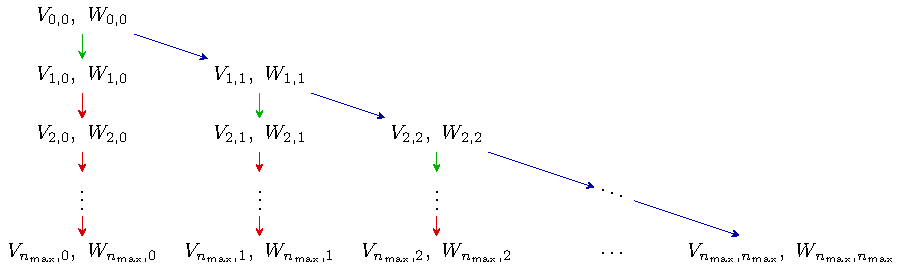
\includegraphics[width=\textwidth]{Images/scheme_recursion.pdf}
  \caption{Scheme for the calculation of the coefficients $V_{n,m}$ and $W_{n,m}$ for $0\leq m\leq n\leq n_\mathrm{max}$. The red arrows indicate that the coefficients are calculated using the first of the above recursions; the green arrows indicate that they are calculated using the second recursion; and the blue arrows indicate that they are calculated using the third recursion.}
  \label{fig:SHcoeffs}
\end{figure}
\subsection{Other perturbations}
So far we have only considered one force acting on the satellite: the gravitational force exerted by the Earth. However, there are other important forces worth-considering, and they relative importance varies depending on the satellite's altitude.

\subsubsection{Atmospheric drag}
For \emph{LEO} (\emph{Low Earth Orbit}) satellites, that is, satellites with an altitude of less than $1\,000$ km, the most important perturbation is the atmospheric drag. Indeed, as these satellites travel in the upper layers of the atmosphere, they are subject to a drag force caused by the interaction with air particles. The acceleration due to drag can be written as:
\begin{equation}
  \vf{a}_{\mathrm{D}}=-\frac{1}{2}C_{\mathrm{D}}\frac{A}{m}\rho v_r\vf{v}_r
\end{equation}
where $A$ is the cross-sectional area of the satellite, $m$ is its mass, $\rho$ is the atmospheric density, $\vf{v}_r$ is the relative velocity between the satellite and the air particles, $v_r=\norm{\vf{v}_r}$, and $C_{\mathrm{D}}$ is the drag coefficient, which depends on the shape of the satellite and the properties of the air particles. In order to determine $\vf{v}_r$, we will suppose that the atmospheric particles rotate with the Earth, and thus the relative velocity is given by:
\begin{equation}
  \vf{v}_r=\dot{\vf{r}}-\vf{\omega}_\oplus\times\vf{r}
\end{equation}
where $\vf{\omega}_\oplus$ is the angular velocity of the Earth.

The complexity of modeling this force arises from the challenge of representing accurately the atmospheric density as a function of the altitude. We will not delve into this topic, but in the simulation we will use the density model of Harris-Priester, which is valid for altitudes between 100 and $1\,000$ km (see \cite{montenbruck} for more details).

\subsubsection{Sun and Moon gravitational perturbations}
For \emph{MEO} (\emph{Medium Earth Orbit}) satellites, within an altitude between $1\,000$ and $35\,780$ km \cite{vallado}; \emph{GEO} (\emph{Geostationary Earth Orbit} or \emph{Geosynchronous Earth Orbit}) satellites, with an altitude of around $35\,780$ km; and \emph{HEO} (\emph{High Earth Orbit}) satellites, with an altitude of more than $35\,780$ km, the most important perturbations are the gravitational perturbations caused by the Moon and the Sun, or even other celestial bodies.

Adding a third body into the equations requires some carefulness. We will do the general deduction to make it clear for the reader. Suppose we have $N+2$ bodies of masses $M$, $M_1,\ldots, M_N$ and $m\ll M,M_1,\ldots,M_N$ at positions $\vf{s}$, $\vf{s}_1,\ldots,\vf{s}_N$ and $\vf{r}$, respectively, in an inertial reference frame (we omit the dependence in time). The dynamics of this system are governed by the following system of differential equations:
\begin{equation}
  \begin{cases}
    \displaystyle \ddot{\vf{s}}=\sum_{i=1}^N\frac{GM_i}{\norm{\vf{s}_i-\vf{s}}^3}(\vf{s}_i-\vf{s})      +\frac{Gm}{\norm{\vf{r}-\vf{s}}^3}(\vf{r}-\vf{s}) \\
    \displaystyle \ddot{\vf{s}}_i=\frac{GM}{\norm{\vf{s}-\vf{s}_i}^3}(\vf{s}-\vf{s}_i)+\sum_{\substack{j=1                                                \\j\ne i}}^N\frac{GM_j}{\norm{\vf{s}_j-\vf{s}_i}^3}(\vf{s}_j-\vf{s}_i)+\frac{Gm}{\norm{\vf{r}-\vf{s}_i}^3}(\vf{r}-\vf{s}_i)& \text{for } i=1,\ldots, N \\
    \displaystyle \ddot{\vf{r}}=\frac{GM}{\norm{\vf{s}-\vf{r}}^3}(\vf{s}-\vf{r})+\sum_{i=1}^N\frac{GM_i}{\norm{\vf{s}_i-\vf{r}}^3}(\vf{s}_i-\vf{r})
  \end{cases}
\end{equation}
Here $G$ is the gravitational constant. Since $m\ll M,M_1,\ldots,M_N$, we can assume that the motion of the large bodies is not affected by the small body, i.e.\ we can make $m$ tend to zero and assume:
\begin{equation}
  \begin{cases}
    \displaystyle \ddot{\vf{s}}= \sum_{i=1}^N\frac{GM_i}{\norm{\vf{s}_i-\vf{s}}^3}(\vf{s}_i-\vf{s})        \\
    \displaystyle \ddot{\vf{s}}_i=\frac{GM}{\norm{\vf{s}-\vf{s}_i}^3}(\vf{s}-\vf{s}_i)+\sum_{\substack{j=1 \\j\ne i}}^N\frac{GM_j}{\norm{\vf{s}_j-\vf{s}_i}^3}(\vf{s}_j-\vf{s}_i)& \text{for } i=1,\ldots, N \\
    \displaystyle \ddot{\vf{r}}=\frac{GM}{\norm{\vf{s}-\vf{r}}^3}(\vf{s}-\vf{r})+\sum_{i=1}^N\frac{GM_i}{\norm{\vf{s}_i-\vf{r}}^3}(\vf{s}_i-\vf{r})
  \end{cases}
\end{equation}
For our purposes, if the body of mass $M$ is the Earth and the body of mass $m$ is the satellite, we are interested in the position of the satellite relative to the Earth, that is $\vf{R}=\vf{r}-\vf{s}$. The dynamics of $\vf{R}$ is governed by the following equation:
\begin{equation}
  \ddot{\vf{R}}=-\frac{GM}{\norm{\vf{R}}^3}\vf{R}+\sum_{i=1}^N\frac{GM_i}{\norm{\vf{s}_i-\vf{s}-\vf{R}}^3}(\vf{s}_i-\vf{s}-\vf{R})-\sum_{i=1}^N\frac{GM_i}{\norm{\vf{s}_i-\vf{s}}^3}(\vf{s}_i-\vf{s})
\end{equation}
Taking the origin of the inertial reference frame at the center of mass of the Earth, i.e.\ $\vf{s}=0$, the latter equation finally becomes:
\begin{equation}
  \ddot{\vf{R}}=-\frac{GM}{\norm{\vf{R}}^3}\vf{R}+\sum_{i=1}^N\frac{GM_i}{\norm{\vf{s}_i-\vf{R}}^3}(\vf{s}_i-\vf{R})-\sum_{i=1}^N\frac{GM_i}{\norm{\vf{s}_i}^3}\vf{s}_i=-\frac{GM}{\norm{\vf{R}}^3}\vf{R}+\sum_{i=1}^N\vf{a}_i
\end{equation}
where $\vf{a}_i=\frac{GM_i}{\norm{\vf{s}_i-\vf{R}}^3}(\vf{s}_i-\vf{R})-\frac{GM_i}{\norm{\vf{s}_i}^3}\vf{s}_i$ is the contribution of the $i$-th body to the acceleration of the satellite.
In the simulation, we will replace the first term of the right-hand side of the equation by the expansion of the acceleration in spherical harmonics.

\subsubsection{Solar radiation pressure}
Satellites in medium and high-altitude orbits may also experience a force that arises from the absortion or reflection of photons emitted by the Sun \cite{montenbruck}. We will expose a brief overview on how this solar radiation pressure is modeled and how it is included in the equations of motion. The acceleration due to solar radiation pressure is given by:
\begin{equation}\label{eq:preSolarRad}
  {\vf{a}}_{\mathrm{R}}=-P_{\odot} C_{\mathrm{R}} \frac{A_\odot}{m} \frac{\vf{s}_\odot-\vf{r}}{\norm{\vf{s}_\odot-\vf{r}}}
\end{equation}
Here $P_{\odot}= 4.57\times 10^{-6}\ \N / \m^2$ is the solar radiation pressure at around the distance of the Earth, $C_{\mathrm{R}}=1+\varepsilon\in [0,2]$ is the radiation pressure coefficient and $\varepsilon$ is the reflectivity coefficient, being $C_{\mathrm{R}}=0$ for a perfectly translucent body, $C_{\mathrm{R}}=1$ for a perfectly absorbing body, and $C_{\mathrm{R}}=2$ for a perfectly reflecting body. $\vf{r}$ denotes the position of the satellite relative to the Earth, $\vf{s}_\odot$ is the position of the Sun relative to the Earth, $m$ the mass of the satellite and $A_\odot$ its fraction of area exposed to the Sun.

One should note that $A_\odot$ and $A$ (the cross-sectional area of the satellite used to compute the drag force) are in general not the same. We will see in the next section, though, that due to the difficulties on determining them, we will assume that they are equal and constant throughout the integration process.

In reality, \cref{eq:preSolarRad} does not describe entirely well the perturbation due to the solar radiation. Indeed, an illumination factor $\nu\in[0,1]$ should be added into the equation to account for the fraction of solar rays that actually reach the satellite. This cause the disctinction of three regions: the illumination zone ($\nu=1$), where the satellite is fully exposed to the Sun; the penumbral zone ($0<\nu<1$), where the satellite is partially exposed to the Sun, and the umbral zone ($\nu=0$), where the satellite receives no solar radiation due to the Earth obstructing the light.
Thus, \cref{eq:preSolarRad} should be corrected to:
\begin{equation}\label{eq:SolarRad}
  {\vf{a}}_{\mathrm{R}}=-\nu P_{\odot} C_{\mathrm{R}} \frac{A_\odot}{m} \frac{\vf{s}_\odot-\vf{r}}{\norm{\vf{s}_\odot-\vf{r}}^3}
\end{equation}
\cref{fig:penumbra} shows a 2D schematic representation of the penumbra and umbral zones of the Earth. To determine whether the satellite is or not inside on of these zones, we must compute the dot product between $\vf{r}$ and $\vf{s}_\odot$ and if it is negative, then compare the relative ``altitude'' of the satellite with respect to the ``altitudes'' of the penumbral and umbral zones ($y_\mathrm{sat}$, $y_{\mathrm{pen}}$ and $y_{\mathrm{umb}}$ respectively in the figure).
\begin{figure}[ht]
  \centering
  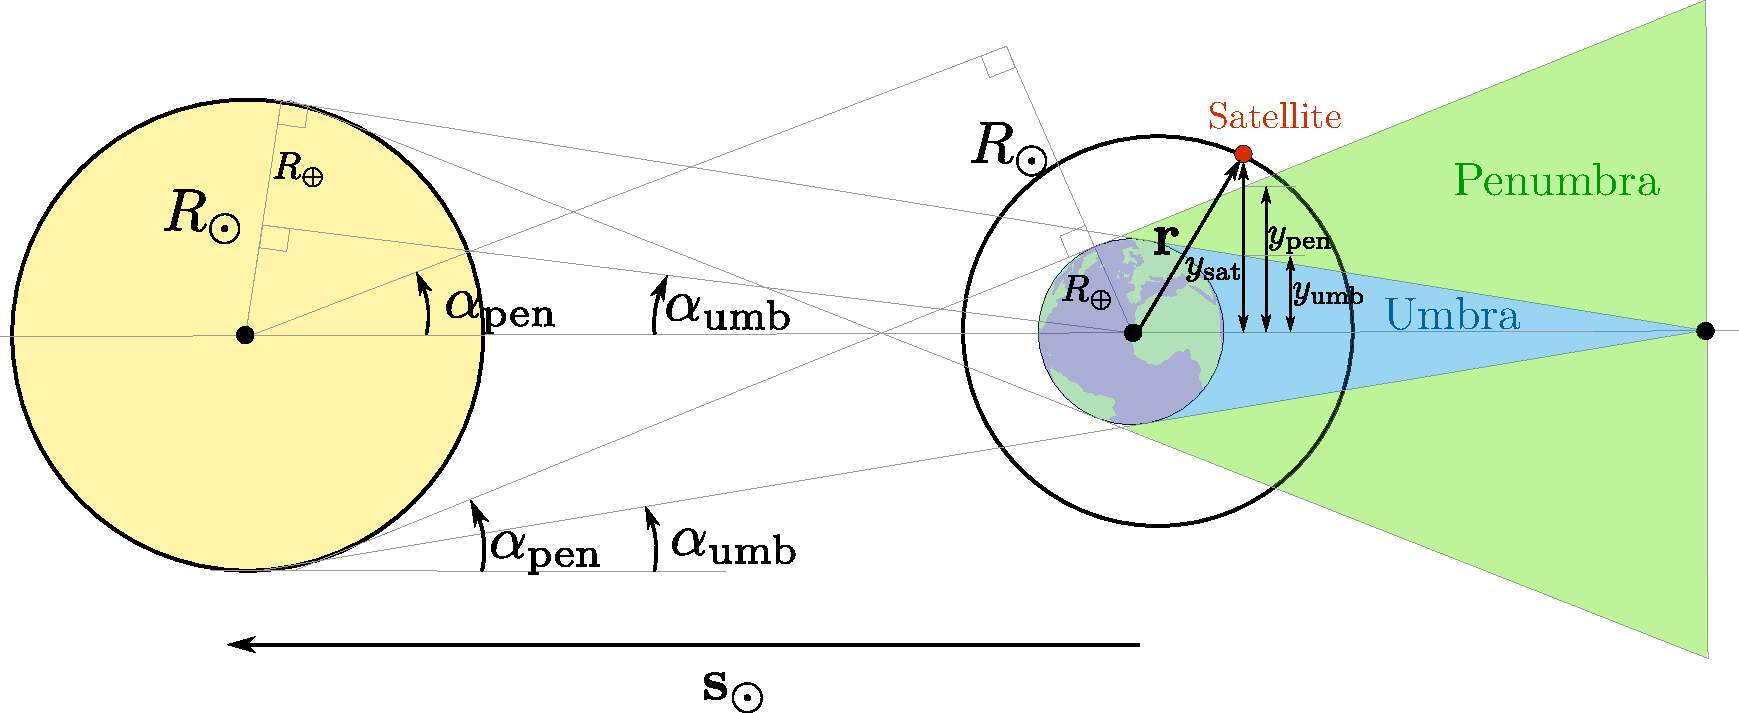
\includegraphics[width=0.8\textwidth]{Images/penumbra.pdf}
  \caption{Schematic representation of the penumbra and umbral zones. Based on \cite{vallado}.}
  \label{fig:penumbra}
\end{figure}
\subsubsection{Minor perturbations}
In addition to the major perturbations described above, there are other minor perturbations that we will not consider in this work, but they are worth-considering if accurate results are required. Some of these perturbations include the perturbations caused by other planets, relativistic effects, the Earth tide effects, or radiation pressure caused by the sunlight reflected by the Earth (albedo) \cite{montenbruck}.
% From  https://physics.stackexchange.com/questions/19477/earth-centered-inertial-eci-reference-frame-as-approximate-inertial-frame-of-r
% ECI coordinate frames are not truly inertial since the Earth itself is accelerating as it travels in its orbit about the Sun. In many cases, it may be assumed that the ECI frame is inertial without adverse effect. However, when computing the gravitational influence of a third body such as the Moon on the dynamics of a spacecraft, the acceleration of the ECI frame must be considered. For example, when computing the acceleration of an Earth-orbiting spacecraft due to the gravitational influence of the Moon, the acceleration of the Earth itself due to the Moon's gravity must be subtracted
\end{document}